\documentclass[../notas medios.tex]{subfiles}
\begin{document}

\chapter{Elasticidad}


\graphicspath{{img/Cap6/}}
\section{Introducción}

Al final de esta sección el estudiante deberá estar en la capacidad de
\begin{itemize}
\item[•] Entender las hipótesis básicas de la elasticidad lineal.
\item[•] Reconocer la relación de tensión-deformación para materiales elásticos lineales.
\item[•] Identificar los efectos físicos relacionados con las constantes de material como el módulo de Young y el coeficiente de Poisson.
\item[•] Identificar las consideraciones implicadas en las idealizaciones de esfuerzo plano y deformación plana.
\item[•] Operar en problemas de elasticidad simples.
\end{itemize}

Como se discutió en el capítulo 5 las condiciones de equilibrio en términos de tensiones se reducen a 3 ecuaciones diferenciales parciales en las 9 componentes del tensor de tensiones y a 3 relaciones de simetría resultantes del equilibrio rotacional del punto material: en total estas correspondían a 6 ecuaciones en 9 incógnitas. Al introducir los cambios cinemáticos en términos del tensor de deformaciones unitarias se involucran en el problema las siguientes 6 ecuaciones adicionales y 9 incógnitas más
\begin{align*}
&\varepsilon_{xx} = \frac{\partial u}{\partial x}\, ,\quad
\varepsilon_{yy} = \frac{\partial v}{\partial y}\, ,\quad
\varepsilon_{zz} = \frac{\partial w}{\partial z}\, ,\\
&\varepsilon_{xy} = \frac{1}{2}\left(\frac{\partial u}{\partial y} + \frac{\partial v}{\partial x} \right)\, ,\quad
\varepsilon_{xz} = \frac{1}{2}\left(\frac{\partial u}{\partial z} + \frac{\partial w}{\partial x} \right)\, ,\quad
\varepsilon_{yz} = \frac{1}{2}\left(\frac{\partial v}{\partial z} + \frac{\partial w}{\partial y} \right)\, ,
\end{align*}
con lo que se tienen en total 12 ecuaciones en 18 incógnitas.

Aunque todos los problemas abordados hasta el momento han estado relacionados con sólidos, también es cierto que en ningún momento hemos hecho distinción alguna de un material a otro. Es decir las soluciones en términos de tensiones para problemas como el de la cuña autosoportada son igualmente válidas independientemente del material del que este fabricada la cuña. En esta sección se presentan  relaciones entre las tensiones y las deformaciones las cuales cambiarán necesariamente de un material a otro. Por ejemplo, refiriéndonos al problema de la cuña, es natural esperar que si 2 cuñas con iguales geometrías y sometidas a los mismos cortantes de magnitud $S$, pero fabricadas de 2 materiales diferentes, por ejemplo acero y madera, éstas se deformen en magnitudes diferentes. De forma general podemos escribir estas relaciones como
\begin{equation}
\left\{ \begin{array}{*{20}{c}}
\sigma_{xx}\\
\sigma _{yy}\\
\sigma _{zz}\\
\tau_{xy}\\
\tau_{xz}\\
\tau_{yz}
\end{array} \right\} = \left[ \begin{array}{*{20}{c}}
C_{11} &C_{12} &C_{13} &C_{14} &C_{15} &C_{16}\\
C_{21} &C_{22} &C_{23} &C_{24} &C_{25} &C_{26}\\
C_{31} &C_{32} &C_{33} &C_{34} &C_{35} &C_{36}\\
C_{41} &C_{42} &C_{43} &C_{44} &C_{45} &C_{46}\\
C_{51} &C_{52} &C_{53} &C_{54} &C_{55} &C_{56}\\
C_{61} &C_{62} &C_{63} &C_{64} &C_{65} &C_{66}
\end{array} \right]\left\{ \begin{array}{*{20}{c}}
\varepsilon_{xx}\\
\varepsilon_{yy}\\
\varepsilon_{zz}\\
\varepsilon_{xy}\\
\varepsilon_{xz}\\
\varepsilon_{yz}
\end{array} \right\}.
\label{conselas}
\end{equation}

Con la \cref{conselas} se tienen ahora 18 ecuaciones en 18 incógnitas con lo cual la solubilidad o no del problema depende ahora de las condiciones especificadas en la frontera.

\section{Hipótesis básicas}
En esta sección se particulariza el modelo del medio continuo al modelo más simple: un sólido elástico lineal. Las hipótesis básicas para la teoría de elasticidad lineal son:
\begin{itemize}
\item \textbf{El material es elástico.} Esto implica que el cuerpo retorna a su estado inicial cuando las fuerzas externas dejan de actuar sobre él. Esto implica que el trabajo realizado sobre el cuerpo se almacena como energía de deformación y que no hay disipación de energía en este proceso.

\item \textbf{Los materiales son isótropos.} Esto implica que las propiedades de los materiales no dependen de la dirección en la que se midan. Por ejemplo, la madera no es un material isótropo, pues las propiedades mecánicas son diferentes en la dirección de la fibra que perpendicular a esta.

\item \textbf{Los materiales son homogéneos.} Esto implica que las propiedades de los materiales son iguales en todos los puntos del medio.

\item \textbf{Los materiales son lineales.} Un material es lineal si las deformaciones pueden escribirse como una relación lineal de las tensiones, es decir, si satisface la \cref{conselas}.

\item \textbf{Las deformaciones son pequeñas.} Esto implica que las ecuaciones de equilibrio son válidas en la configuración inicial del medio.

\end{itemize}

Estas consideraciones hacen que la \cref{conselas} se simplifique enormemente, y que la cantidad de constantes involucradas se reduzcan de 36 a 2.

\section{Relación tensión-deformación}
Considerando las hipótesis planteadas en el párrafo anterior las relaciones de la  \cref{conselas} se reducen a las relaciones tensión - deformación dadas en la  \cref{esfdef}:

\begin{equation} \label{esfdef}
\begin{split}
& \sigma_{xx} = \dfrac{E}{(1 + \nu)} \varepsilon_{xx} + \dfrac{\nu E}{(1 + \nu)(1-2 \nu)} (\varepsilon_{xx} + \varepsilon_{yy} + \varepsilon_{zz}) \\
& \sigma_{yy} =\dfrac{E}{(1 + \nu)} \varepsilon_{yy} + \dfrac{\nu E}{(1 + \nu)(1-2 \nu)} (\varepsilon_{xx} + \varepsilon_{yy} + \varepsilon_{zz}) \\
& \sigma _{zz} = \dfrac{E}{(1 + \nu)} \varepsilon_{zz} + \dfrac{\nu E}{(1 + \nu)(1-2 \nu)} (\varepsilon_{xx} + \varepsilon_{yy} + \varepsilon_{zz}) \\
& \tau_{xy} = G \gamma_{xy}  \\
& \tau_{xz} = G \gamma_{xz}  \\
& \tau_{zy} = G \gamma_{yz}
\end{split}
\end{equation}

y  las relaciones deformación - tensión dadas en la \cref{defesf}:
\begin{equation} \label{defesf}
\begin{split}
& \varepsilon_{xx} = \frac{1}{E}\left[ \sigma_{xx} - \nu (\sigma_{yy} + \sigma_{zz})\right] \\
& \varepsilon_{yy} = \frac{1}{E}\left[ \sigma_{yy} - \nu (\sigma_{xx} + \sigma_{zz}) \right] \\
& \varepsilon_{zz} = \frac{1}{E}\left[ \sigma_{zz} - \nu (\sigma_{xx} + \sigma_{yy}) \right] \\
& \gamma_{xy} = \frac{\tau_{xy}}{G} \\
& \gamma_{xz} = \frac{\tau_{xz}}{G} \\
& \gamma_{zy} = \frac{\tau_{zy}}{G}\, ,
\end{split}
\end{equation}

En la \cref{esfdef} y en la \cref{defesf}, conocidas comúnmente como la Ley de Hooke, las constantes $E$ (módulo elástico o de módulo de Young) , $G$ (módulo elástico de cortante) y $\nu$ (relación de Poisson) son propias de cada material. El valor de dichas constantes se puede determinar mediante ensayos de laboratorio de tensión simple para el módulo elástico $E$ y relación de Poisson $\nu$ y de torsión pura para el módulo de cortante $G$. Por otro lado es posible hallar la siguiente relación entre constantes.
\[G = \dfrac{E}{2(1 + \nu)}\]

\section{Idealizaciones en 2D}

En general, es difícil resolver problemas en 3D. Por esta razón, existen varias idealizaciones que consideran el medio continuo como si este fuera plano. Estas simplificaciones consideran que:
\begin{itemize}
\item[•] el medio está acotado por dos superficies planas paralelas al plano \(xy\);
\item[•] la sección transversal del medio es uniforme en la dirección \(z\);
\item[•] la carga se distribuye uniformemente en la dirección \(z\); y
\item[•] no hay tracciones tangenciales en las superficies planas que acotan el medio.
\end{itemize}
Debemos resaltar que la tercera restricción implica que no habrá torsión. Estas restricciones no implican, sin embargo, que el medio continuo debe ser delgado.

Las variables involucradas en las idealizaciones planas son reducidas a 2 desplazamientos y 3 esfuerzos/deformaciones. Específicamente:
\begin{itemize}
\item[] Desplazamientos: \(u\), \(v\);
\item[] Deformaciones: \(\varepsilon_{xx}\), \(\varepsilon_{yy}\), \(\gamma_{xy}\); 
\item[] Esfuerzos: \(\sigma_{xx}\), \(\sigma_{yy}\), \(\tau_{xy}\);
\end{itemize}
en coordenadas cartesianas y
\begin{itemize}
\item[] Desplazamientos: \(u_r\), \(u_\theta\);
\item[] Deformaciones: \(\varepsilon_{rr}\), \(\varepsilon_{\theta\theta}\), \(\gamma_{r\theta}\); 
\item[] Esfuerzos: \(\sigma_{rr}\), \(\sigma_{\theta\theta}\), \(\tau_{r\theta}\);
\end{itemize}
en coordenadas polares.


\subsection{Tensión plana}
Decimos que un medio continuo está en tensión plana (o esfuerzo plano) si el estado de esfuerzos es tal que una de sus componentes principales es cero en todo el medio. Podemos elegir esta dirección principal alineada con \(z\), lo que implica \(\sigma_{zz}=\sigma_{xz}=\sigma_{yz}=0\) en todo el cuerpo. Esta idealización es común para placas delgadas con cargas paralelas a las caras. En algunos casos, se puede considerar como tensión plana placas levemente curvadas. Este es el caso de un cilindro con pared delgada bajo la acción de una presión, como en un tanque.

Las relaciones deformación-tensión en este caso se reducen a
\begin{equation} \label{platension}
\begin{split}
& \varepsilon_{zz} =  - \frac{\nu }{E}(\sigma_{xx} + \sigma_{yy}) \\
& \varepsilon_{xx} =    \frac{1}{E}(\sigma_{xx} - \nu \sigma_{yy})\\
& \varepsilon_{yy} = \frac{1}{E}(\sigma_{yy} - \nu \sigma_{xx})\\
& \gamma_{xy} = \frac{\tau_{xy}}{G}
\end{split}
\end{equation}

Note que \(\varepsilon_{zz} \neq 0\), sin embargo, puede prescindirse de él para el análisis, pues puede obtenerse a partir de los esfuerzos/deformaciones en el plano.


\subsection{Deformación plana}
Decimos que un medio continuo está en deformación plana si el estado de deformaciones es tal que una de sus componentes principales es cero en todo el medio. Podemos elegir esta dirección principal alineada con \(z\), lo que implica \(\varepsilon_{zz}=\varepsilon_{xz}=\varepsilon_{yz}=0\) en todo el cuerpo. Esta idealización es común para cuerpos que tienen una dimensión muy grande comparada las demás.

Las relaciones de deformación esfuerzo deformación para las componentes axiales serían entonces
\begin{align*}
&\varepsilon_{xx} = \frac{1}{E}\left[\sigma_{xx} - \nu (\sigma_{yy} + \sigma_{zz}) \right]\\
&\varepsilon_{yy} = \frac{1}{E}\left[\sigma_{yy} - \nu (\sigma_{xx} + \sigma_{zz}) \right]\\
&0 = \frac{1}{E}\left[\sigma_{zz} - \nu (\sigma_{xx} + \sigma_{yy}) \right]
\end{align*}
de donde
\[\sigma_{zz} = \nu (\sigma_{xx} + \sigma_{yy})\]

Eliminando $\sigma _{zz}$ se tiene que:
\begin{equation} \label{plastrain}
\begin{split}
& {\varepsilon _{xx}} = \frac{{1 - {\nu ^2}}}{E}{\sigma _{xx}} - \frac{{\nu (1 + \nu )}}{E}{\sigma _{yy}} \\
& {\varepsilon _{yy}} = \frac{{1 - {\nu ^2}}}{E}{\sigma _{yy}} - \frac{{\nu (1 + \nu )}}{E}{\sigma _{xx}} \\
& {\gamma _{xy}} = \frac{{{\tau _{xy}}}}{G}
\end{split}
\end{equation}

\subsubsection{Reescritura como tensión plana}
Es posible escribir las formulaciones de tensión plana y deformación plana de manera equivalente. En el caso de deformación plana, si se introduce los siguientes módulos equivalente
\[\bar E = \frac{E}{1 - \nu^2}\]
y
\[\bar \nu  = \frac{\nu }{1 - \nu}\, ,\]
podemos escribir las relaciones de deformación-tensión como
\begin{align*}
& \varepsilon_{zz} =  - \frac{\bar\nu}{\bar E}(\sigma_{xx} + \sigma_{yy}) \\
& \varepsilon_{xx} =    \frac{1}{\bar E}(\sigma_{xx} - \bar\nu \sigma_{yy})\\
& \varepsilon_{yy} = \frac{1}{\bar E}(\sigma_{yy} - \bar\nu \sigma_{xx})\\
& \gamma_{xy} = \frac{\tau_{xy}}{G}\, ,
\end{align*}
note que el módulo de cortante \(G\) no se ve afectado por esta transformación.

\section{Ejemplos resueltos}
\subsection*{Ejemplo 1: Cuña autosoportada}

Regresando al ejemplo de la cuña auto-soportada (\cref{wedgee})
\begin{figure}[H]
\centering
	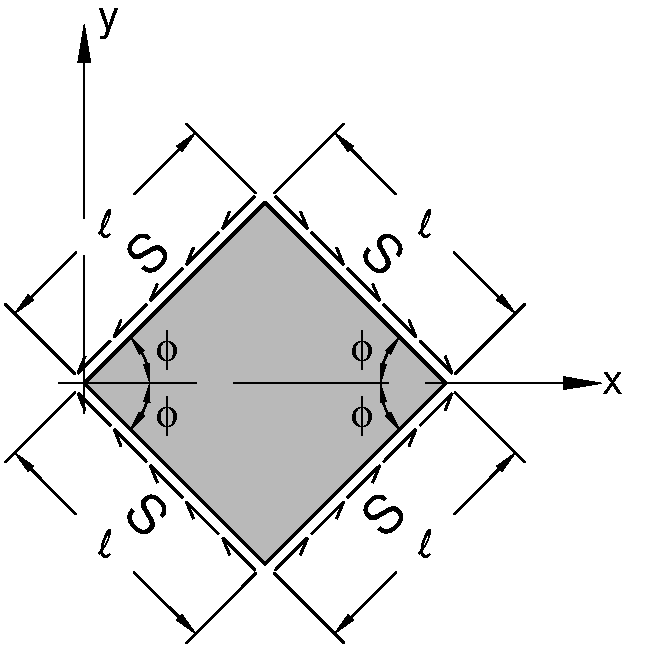
\includegraphics[width=2.8 in]{wedge.pdf}
	\caption{Cuna auto-soportada.}
	\label{wedgee}
\end{figure}


Usando argumentos de equilibrio determinamos que el campo de tensiones solución del problema estaba dado por:
\begin{equation} \label{tencuna}
\begin{split}
& \sigma_{xx} = S \cot\phi \\
& \sigma_{yy} =  - S \tan\phi \\
& \tau_{xy} = 0
\end{split}
\end{equation}

Usando las relaciones tensión-deformación para tensión plana (o deformación plana con módulos efectivos) se tiene que:
\begin{align*}
&\varepsilon_{xx} = \frac{1}{E}[S \cot\phi  + \nu S \tan\phi]\\
&\varepsilon_{yy} =  - \frac{1}{E}[S \tan\phi  + \nu S \cot\phi]
\end{align*}

Recordando las relaciones:
\[\left\{ d\vec u \right\} = \left[ \varepsilon  \right] \cdot \left\{ d\vec x \right\} + \left[ \omega  \right] \cdot \left\{ d\vec x\right\}\]
las cuales para el caso plano se simplifican a
\begin{align*}
&du = \varepsilon_{xx}dx + \frac{\gamma_{xy}}{2}dy - \frac{\omega_{xy}}{2}dy\\
&dv = \varepsilon_{yy}dy + \frac{\gamma_{xy}}{2}dx + \frac{\omega_{xy}}{2}dx
\end{align*}
y reconociendo que por la simetría del problema las componentes rotacionales son nulas se tiene que
\[u = \int \frac{1}{E}[ S \cot\phi  + \nu S \tan\phi]dx  \equiv \frac{1}{E}[S \cot\phi  + \nu S \tan\phi]x + A\]
y
\[v =  - \int \frac{1}{E}[S \tan\phi  + \nu \cot\phi]dy  \equiv  - \frac{1}{E}[S \tan\phi  + \nu S \cot\phi]y + B\]
donde $A$ y $B$ son constantes de integración.


\subsection*{Ejemplo 2: Barra sometida a carga axial}

En la \cref{compresion} se muestra una barra de sección rectangular con $a= 40$ cm, $b = 50$ cm y longitud inicial $L_{c} = 500$ cm, que es  sometida a un ensayo de compresión confinada (está contenida en un recipiente indeformable), mientras que en la \cref{traccion}  se muestra una barra de sección circular con diámetro $d = 50$ cm y longitud inicial $L_{t} = 497$ cm sobre la cual se realiza  un ensayo de tracción simple. Las constantes del material, tanto para la barra rectangular como para la barra circular, son $E=150000$ kgf/cm$^2$ y $\nu=0.20$.

Ambos ensayos se realizan con su extremo fijo  en el plano $z = 0$ y están cargados con un sistema que no transmite esfuerzos cortantes y que hace que el esfuerzo axial se distribuya uniformemente sobre la superficie transversal de las barras. Los esfuerzos que se inducen a las barras varían con el tiempo conforme a lo mostrado en la figura \cref{carga}
\begin{figure}[H]
	\centering
	\subfloat[Barra compresión]{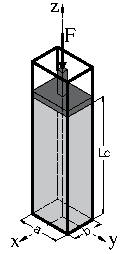
\includegraphics[width=4cm]{Compresion.pdf}\label{compresion}}
	\subfloat[Barra tracción]{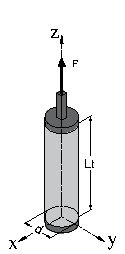
\includegraphics[width=4cm]{Traccion.pdf}\label{traccion}}
	\subfloat[Curvas de esfuerzo]{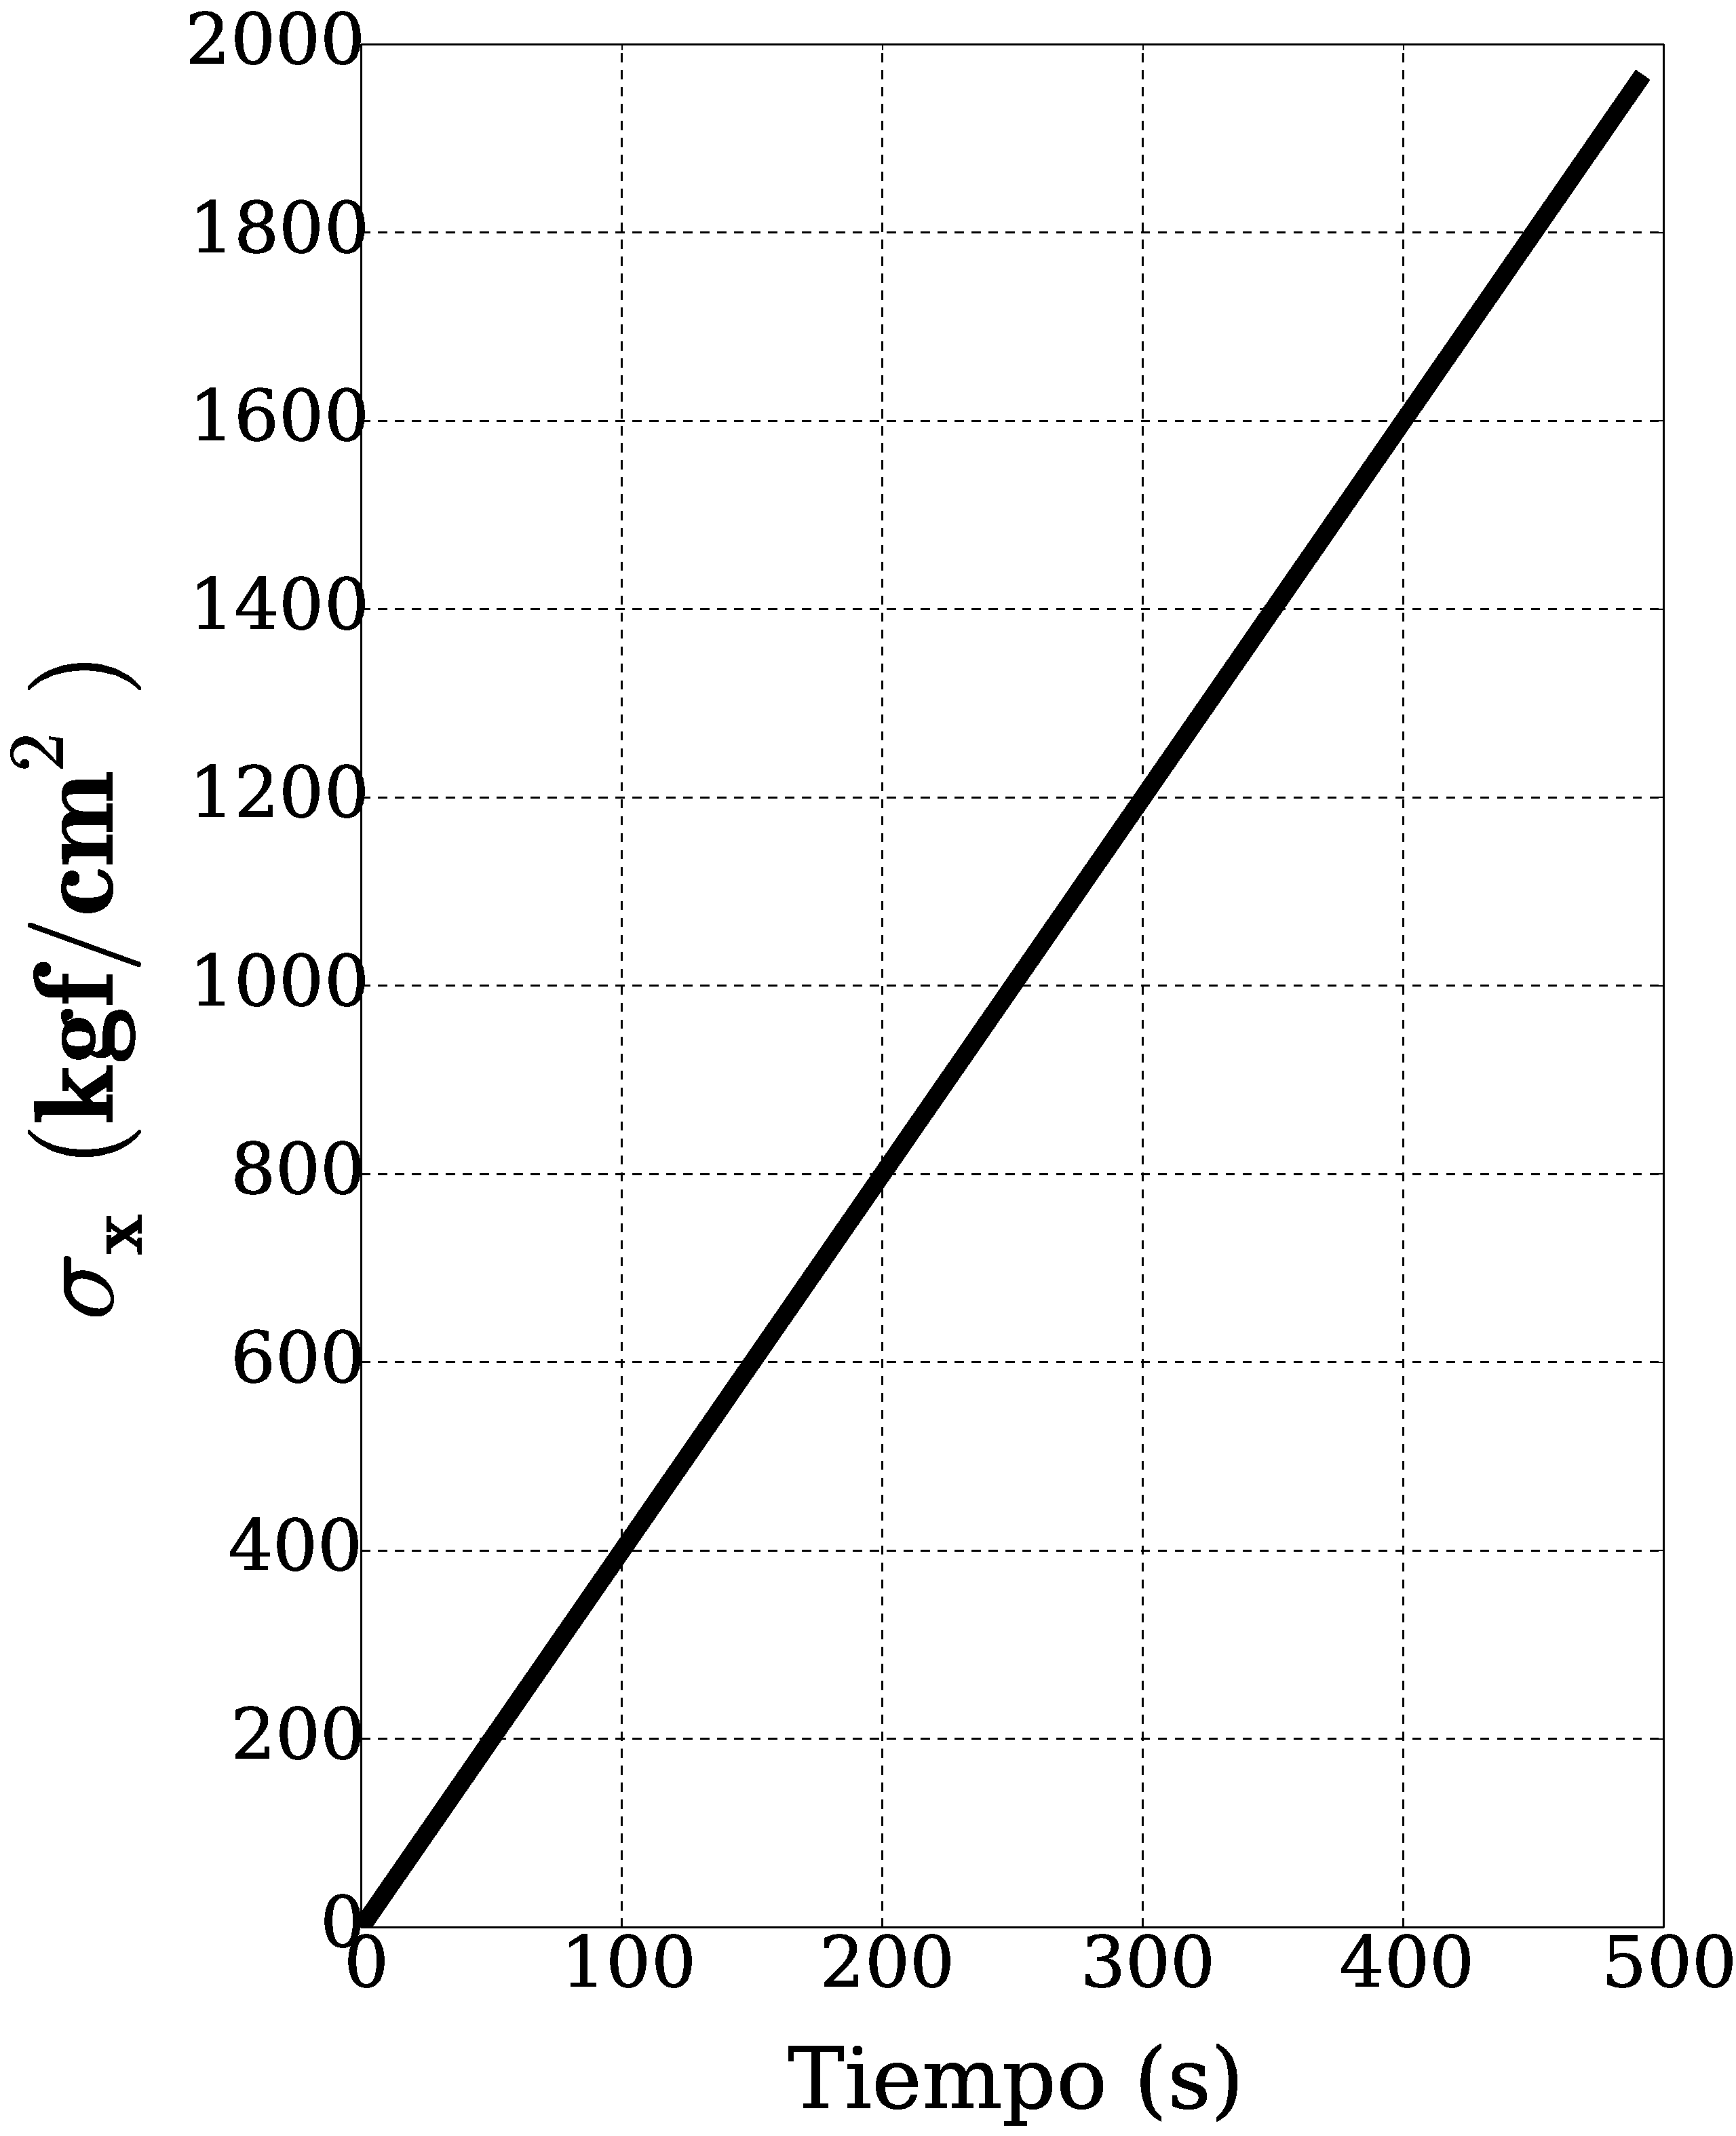
\includegraphics[width=5.5cm]{CurvaEsf.pdf}\label{carga}}
	\caption{Esquema ensayos y curvas de aplicación carga}
	\label{ensayo}
\end{figure}

Determine:
\begin{itemize}
\item ¿Cuál es el tiempo $t$ en el cual las dos barras tienen la misma longitud?

\textbf{Solución:}

La barra circular está solamente sometida a esfuerzo axial $\sigma_{zz}$, por lo que la deformación es
\[\varepsilon _{zz_t} = \dfrac{\sigma_{zz_t} }{E}\, \]
y la longitud final sería:
\begin{equation}
  \begin{split}
  L_{f_{cir}} & = L_{ini_{cir}} (1 +  \varepsilon_{zz_t} )\\
  L_{f_{cir}} & = L_{ini_{cir}} \left(1+  \dfrac{\sigma_{zz_t} }{E}\right)
  \end{split}
  \label{trac}
\end{equation}

Por otro lado, la barra cuadrada está sometida a esfuerzo axial $\sigma_{xx}$, $\sigma_{yy}$ y $\sigma_{zz}$, pero solo se deforma en el eje $z$ que es la deformación de interés. Para este caso entonces,
\[\varepsilon _{zz_c} = \dfrac{\sigma_{zz_c} }{(2 \mu + \lambda)}\]
donde $\mu =   \left(\dfrac{E }{2(1 + \nu)}\right)$  y $\lambda =   \left(\dfrac{\nu{E} }{(1 + \nu) (1 - 2\nu)}\right)$.

Llamando $A = (2 \mu + \lambda)$ se tiene que la longitud final para la barra cuadrada sería:
\begin{equation}
  \begin{split}
  L_{f_{cua}} & = L_{ini_{cua}} (1 +  \varepsilon_{zz_c}) \\
  L_{f_{cua}} & = L_{ini_{cua}} \left(1 +  \dfrac{\sigma_{zz_c} }{A}\right)
  \end{split}
\label{comp}
\end{equation}

Resta, entonces, igualar las longitudes y despejar el tiempo. Para hacer esto, es preciso tener en cuenta barra circular es cargada solo hasta que el esfuerzo es $\sigma=350$ kgf/cm$^2$ por lo que habrá que considerar ambas condiciones. Por simplicidad inicialmente determinemos que pasaría si $t > 350$ s, es decir en donde $\sigma_{zz_t} = 350$  kgf/cm$^2$. Reemplazando el valor de los esfuerzos en función del tiempo en la \cref {trac} y la  \cref{comp}
\begin{equation}
  \begin{split}
  L_{f_{cir}} & = 497 \left(1 +  \dfrac{350 }{E}\right)
  \end{split}
  \label{trac2}
\end{equation}
\begin{equation}
  \begin{split}
  L_{f_{cua}} & = 500 \left(1 - \dfrac{t }{A}\right)
  \end{split}
  \label{comp2}
\end{equation}

donde $A \simeq 1.1111E$.

Igualando la \cref {trac2} y la  \cref{comp2} y despejando $t$ se obtiene
\[t=613.4 \; \text{s}\, .\]

\item En la barra circular, ¿cuáles son los desplazamientos y las deformaciones en el punto de coordenadas $(x,y,z) = (20,15,450)$ cm para el tiempo $t = 300$ s?

Las deformaciones asociadas a la barra son:
\begin{equation}
  \begin{split}
  \varepsilon_{xx_t} &= -\nu \dfrac{\sigma_{zz_t} }{E} \\
  \varepsilon_{yy_t} &= -\nu \dfrac{\sigma_{zz_t} }{E} \\
  \varepsilon_{zz_t} &= \dfrac{\sigma_{zz_t} }{E}
  \end{split}
  \label{defpto2}
\end{equation}
reemplazando $\sigma_{zz_t}$ por 300
\begin{equation}
  \begin{split}
  \varepsilon_{xx_t} &= -0.0004 \\
  \varepsilon_{yy_t} &= -0.0004 \\
  \varepsilon_{zz_t} &= 0.002
  \end{split}
  \label{defpto2sol}
\end{equation}

Por otro lado para determinar los desplazamientos integramos la deformación. Por ser deformación constante la integración se obtiene multiplicando la deformación por las distancias hasta el punto de evaluación.
\begin{equation}
  \begin{split}
  u &= -0.0004 (20  \;\text{cm}) = -0.008 \;\text{cm} \\
  v &= -0.0004 (15  \;\text{cm}) = -0.006 \;\text{cm}  \\
  w &= 0.002  (450  \;\text{cm}) = 0.9  \; \text{cm}\, .
  \end{split}
\label{defpto2sol}
\end{equation}

\item  ¿Cuál es el valor del máximo esfuerzo cortante en un punto al interior de la barra rectangular durante el ensayo?

Los esfuerzos para la barra cuadrada están dados por
\begin{equation}
  \begin{split}
  \sigma_{xx_c} &=   \lambda \varepsilon_{zz_c} \\
  \sigma_{yy_c} &=   \lambda \varepsilon_{zz_c} \\
  \sigma_{zz_c} &=  (2\mu + \lambda) \varepsilon_{zz_c}
  \end{split}
  \label{defpto2}
\end{equation}

El corte máximo se da entonces
\[\tau_{max} = \varepsilon _{zz_c}  \left(\dfrac{2\mu + \lambda - \lambda}{2}\right)\]
llamando de nuevo $A = (2 \mu + \lambda)$,
\[\tau_{max} = \sigma_{zz_c} \left(\dfrac{\mu}{A}\right)\]
para  $\sigma_{zz_c} = 1000 \; \text{kgf/cm}^2$,
\[\tau_{max} = 1000 \left(\dfrac{\mu}{A}\right) \; \text{kgf/cm}^2\, .\]

\end{itemize}

\subsection*{Ejemplo 3: Cilindro sometido a torsión}

Se tiene un cilindro sometido a torsión con un giro por unidad de longitud $2\beta$. El campo de desplazamientos para este problema está dado por
\[
  u = -2\beta zy\, ,\quad
  v = 2\beta zx\, , \quad
  w = 0\, ,
\]
en donde $2\beta = 2\theta/h$, representa el giro por unidad de longitud y está dado en rad/m si los desplazamientos están en m.
\begin{figure}[H]
 \centering
 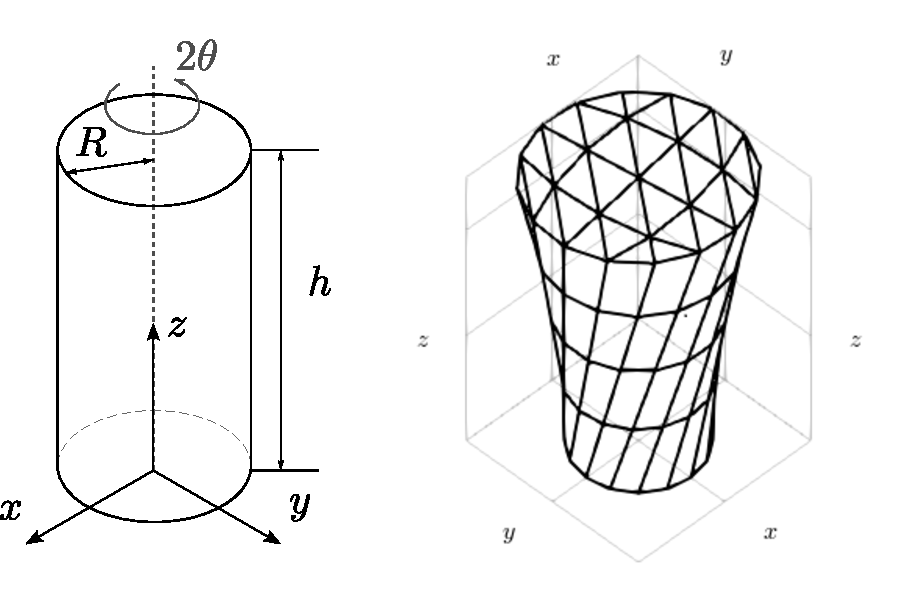
\includegraphics[height=2 in]{cilindro_torsion.pdf} 
 \caption{\textbf{(Izquierda)} Esquema de un cilindro sometido a una torsión en la parte superior y empotrado en la parte inferior. \textbf{(Derecha)} Configuración deformada para el cilindro sometido a torsión. Se dibuja una rejilla sobre el sólido por claridad.}
 \label{fig:cilindro_torsion}
\end{figure}

\begin{itemize}
\item
Si el cilindro debe ir al interior de una cavidad cilíndrica, es decir, el radio de la cavidad debe ser mayor o igual al del cilindro deformado ¿Cuál es el radio interno mínimo de la cavidad si $h=1$ m, $R = 10$ cm y $2\theta = \sqrt{21}/10$ rad?


Para resolver este problema debemos saber cuál es el máximo radio que el cilindro va a tener luego de deformarse, para ello necesitamos la región con mayores desplazamientos. Para saber en dónde ocurren los mayores desplazamientos podemos analizar las ecuaciones de desplazamientos para ver que esto pasa en $z=h$. El campo de desplazamiento allí sería (sin considerar el desplazamiento en $z$ que es nulo):
\[u = -2\theta y,\quad v = 2\theta x\, .\]

Alternativamente, podríamos saber que el mayor desplazamiento pasa en $z=h$ analizando la configuración deformada que se presenta en los anexos.

Adicionalmente, sabemos que el nuevo radio del cilindro estaría dado por la posición de los puntos ubicados en la circunferencia $x^2 + y^2 = R^2$. Estos puntos tienen como ecuaciones paramétricas
\begin{align*}
  x &= R \cos\alpha\, ,\\
  y &= R \sin\alpha\, ,
\end{align*}
en donde $\alpha$ es un parámetro. Tenemos, pues, que la posición de los nuevos puntos de la circunferencia estarían dados por
\begin{align*}
  x_\text{deformado} &= R \cos\alpha - 2R\theta \sin\alpha \, ,\\
  y_\text{deformado} &= R \sin\alpha + 2R\theta \cos\alpha\, .
\end{align*}

Usando el teorema de Pitágoras, podemos calcular la magnitud del nuevo radio
\begin{align*}
  R_\text{deformado}^2 &= x_\text{deformado}^2 + y_\text{deformado}^2\\
    &= [R \cos\alpha - 2R\theta \sin\alpha]^2 + [R \sin\alpha + 2R\theta \cos\alpha]^2\\
    &= 4R^2\theta^2\sin^2\alpha + 4R^2\theta^2\cos^2\alpha + R^2\sin^2\alpha + R^2\cos^2\alpha\\
    &= 4R^2\theta^2[\sin^2\alpha + \cos^2\alpha] + R^2[\sin^2\alpha + \cos^2\alpha]\\
    &= 4R^2\theta^2 + R^2\\
    &= R^2 (1 + 4\theta^2)\, .
\end{align*}
que es equivalente a
\[R_\text{deformado} = R\sqrt{1 + 4\theta^2}\, ,\]
o
\[\frac{R_\text{deformado}}{R} = \sqrt{1 + 4\theta^2}\, .\]

También se pudo haber analizado cómo se movía el punto $(R, 0)$, que en la configuración deformada estaría en $(R, 2\theta R)$. Lo que nos permitiría llegar a la misma conclusión, pero de manera más simple.

Ahora, si $2\theta =\sqrt{21}/10$, entonces $\theta = \sqrt{21}/20$ y tendríamos que
\begin{align*}
  \frac{R_\text{deformado}}{R} &= \sqrt{1 + 4\times \frac{21}{400}} \\
    &= \sqrt{1 + \frac{21}{100}} \\
    &= \sqrt{\frac{121}{100}} \\
    &= \frac{11}{10}\, ,
\end{align*}
Lo que nos permite concluir que el radio máximo es 11 cm.

\item
Si el cilindro está hecho de hormigón, material para el cual se tiene que $\gamma_{\max} = 10^{-4}$ ¿Cuál es el valor máximo de $\theta$ posible antes que el material falle si $R = 1$ m y $h=10$ m?

El tensor de deformaciones unitarias en este caso es
\[[\varepsilon] =\begin{bmatrix}
	0 &0 &-\beta y\\
	0 &0 &\beta x\\
	-\beta y &\beta x &0
    \end{bmatrix}\, .
   \]
   
Para calcular $\gamma_{\max}$ necesitamos encontrar los valores principales de $[\varepsilon]$ (que se pueden hallar como se describe en el anexo). Estos son la solución del polinomio característico
\[\lambda^3 - \lambda \beta^2(x^2 + y^2) = 0\, ,\]
o
\[\lambda^3 - \lambda \beta^2 r^2 = 0\, .\]

Este polinomio puede factorizarse como
\[\lambda[\lambda^2 - \beta^2 r^2] = 0\, ,\]
las raíces son, entonces,
\[\lambda_1 = |\beta r|,\, \lambda_2 = 0,\, \lambda_3 = -|\beta r|\, ,\]
y $\gamma_{\max} = |\beta r| - (-|\beta r|) = 2|\beta r|$. El valor máximo es cuando $r=R$ y tenemos que
\[\gamma_{\max} = 2\beta R\, ,\]
en donde no tuvimos en cuenta el signo de $\beta$, pues este sólo expresa si la torsión se hizo en sentido horario o anti-horario.

Despejando, obtenemos que
\[\theta = \frac{\gamma_{\max}}{2} \left(\frac{h}{R}\right)\, ,\]
y sustituyendo los valores dados
\[\theta = \frac{10^{-4}}{2} \left(\frac{10}{1} \right) = 5\times 10^{-4} \, .\]

\item
Si el cilindro está hecho de acero 1020 con una resistencia al corte \(\tau_\text{cr} = 280 \text{ MPa}\), un módulo de Young de 186 GPa y un coeficiente de Poisson de 0.29
¿Cuál es el valor de par de torsión \(M\) que hace material falle y a qué ángulo de torsión \(\theta_{\max}\) sucede si $R = 20$ mm y $h=1$ m? Use la expresión
\[M = \frac{I_z}{R} \tau_{\max}\, ,\]
para calcular el par de torsión, en donde \(I_z\) es el segundo momento de área para la sección transversal.

Tenemos que \(\tau_{\max} \leq \tau_\text{cr}\), y además \(I_z = \dfrac{\pi R^4}{2}\), luego
\begin{align*}
M &= \frac{\pi R^3}{2}\tau_\text{cr}\\
  &= \frac{\pi \times (20\times 10^{-3}\text{ m})^3 \times 280 \times 10^6 \text{ Pa}}{2}\\
  &= 1120 \pi \text{ N\, m}\\
  &\approx 3518.58 \text{ N\, m}\, .
\end{align*}

Procedemos a calcular el ángulo de torsión al que sucede la falla. A partir de las relaciones de deformación-tensión, tenemos que el esfuerzo está dado por
\[[\sigma] = \beta G\begin{bmatrix}
	0 &0 &-y\\
	0 &0 & x\\
	-y & x &0
    \end{bmatrix}\, ,
   \]
y el esfuerzo cortante máximo estaría dado por \(\tau_{\max} = 2\beta G R\), o
\[\tau_{\max} = \frac{\theta R E}{(1 + \nu) h}\, ,\]
y resolviendo esta ecuación para \(\theta\), obtenemos
\begin{align*}
\theta_{\max} &= \frac{(1 + \nu) h \tau_\text{cr}}{E R} \\
  &= \frac{(1 + 0.29) \text{ m}\times 280\times 10^6 \text{ Pa}}{186\times 10^{9}\text{ Pa} \times 20\times 10^{-3}\text{m}} \\
  &=\frac{301}{3100}\text{ rad}\\
  &\approx 0.097 \text{ rad}\, .
\end{align*}

\end{itemize}


\section{Ejercicios}

\begin{enumerate}

\item \label{punto01_m} Para un campo de desplazamientos dado por:
\[\mathbf{u} = a(x^2 - 5y^2)\hat{\mathbf{i}} + (2ax y)\hat{\mathbf{j}} \]

\begin{enumerate}
\item Determinar el tensor de deformación
\item Obtener las deformaciones principales
\item Obtener los esfuerzos principales
\end{enumerate}

\item \label{punto02_m}  En la  \cref{columna_CargaP} se muestra una columna prismática, de sección cuadrada (lado $a$), con una tracción axial igual a $P$. Si el material del que está hecha la pieza tiene propiedades $\nu$ y $E$, encontrar los campos de esfuerzos y deformaciones.
\begin{figure}[H]
	\centering
	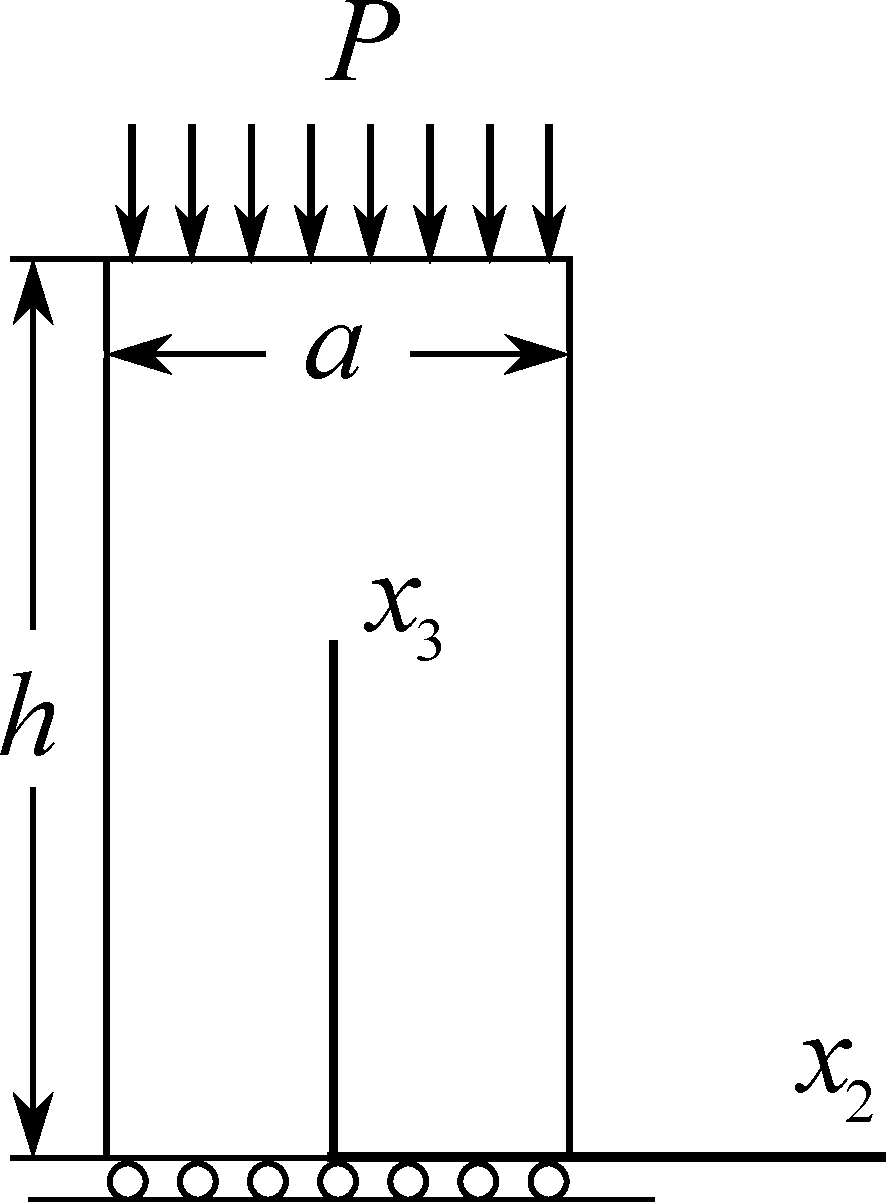
\includegraphics[height=5cm]{columna_CargaP.pdf}
	\caption{Columna con carga axial.}
	\label{columna_CargaP}
\end{figure}

\item \label{punto03_m} En la \cref{fig:columna_g} se muestra la misma columna  del ejercicio anterior, pero en este caso se quiere estudiar la deformación causado por su propio peso. Si las componentes del tensor de esfuerzos son:
\begin{align*}
&\sigma_{33} = \rho g(h- x_{3}) \enspace ,\\
&\sigma_{11} = \sigma_{22} = 0 \enspace ,\\
&\sigma_{12} = \sigma_{13} = \sigma_{23} = 0 \enspace .
\end{align*}

\begin{figure}[h]
	\centering
	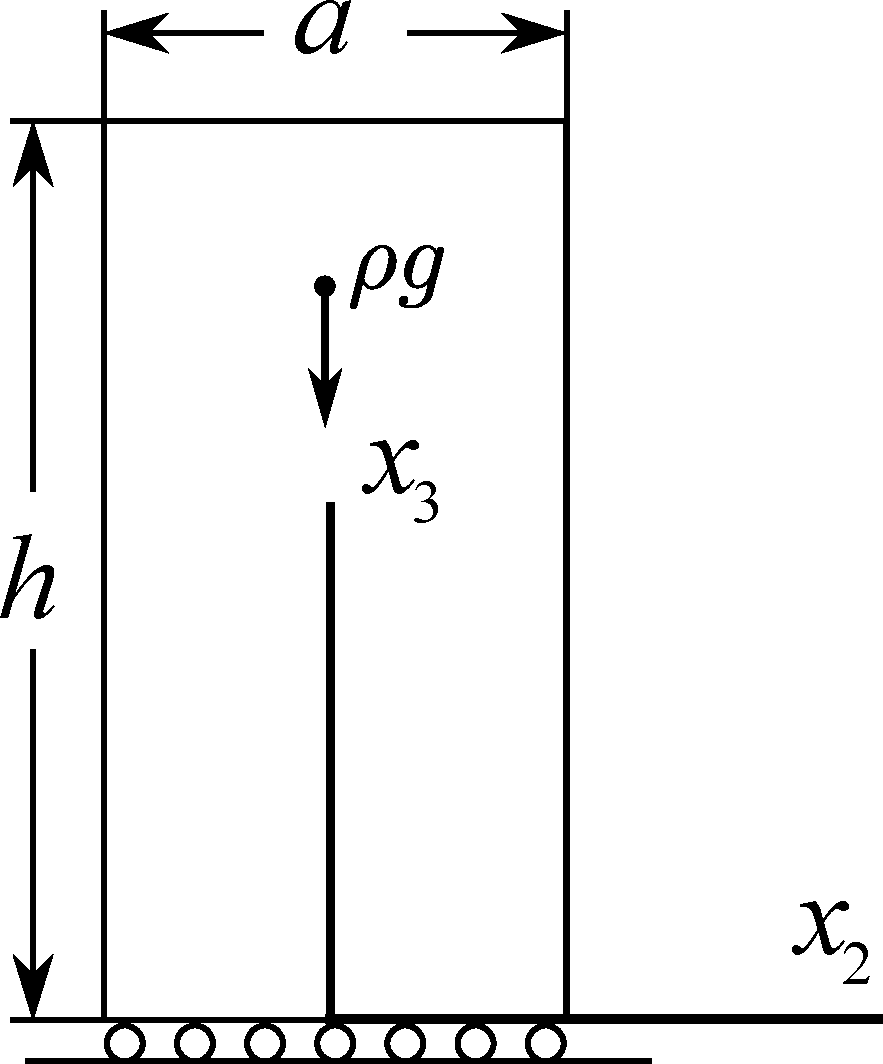
\includegraphics[height=4.5cm]{columna_Peso.pdf}
	\caption{Columna bajo la acción de su propio peso.}
	\label{fig:columna_g}
\end{figure}

\begin{enumerate}
\item Calcular los campos de deformaciones si las propiedades del material son $\nu$ y $E$.
\end{enumerate}


\item \label{punto04_m} En la \cref{fig:viga} se muestra una viga en voladizo de sección unitaria con una carga distribuida en su extremo de forma parabólica.
\[\mathbf{t} = \frac{Pc^2}{2I}\left(1-\frac{y^2}{c^2}\right)\hat{\mathbf{j}}\].La solución para esfuerzos es de la forma
\begin{align*}
&\sigma_{xx} = -\frac{P}{I}xy \enspace ,\\
&\sigma_{yy} = 0 \enspace ,\\
&\sigma_{xy} = -\frac{P}{2I}(c^2 - y^2) \enspace .
\end{align*}

Y para el campo de desplazamientos es:
\begin{align*}
&u_{x} = \left(\frac{1}{G} - \frac{\nu}{E}\right)\frac{Py^3}{6I} + \left(\frac{l^2}{E} - \frac{x^2}{E} - \frac{c^2}{G} \right)\frac{Py}{2I} \enspace ,\\
&u_{y} = \frac{\nu P xy^2}{2EI} + \frac{Px^3}{6EI} - \frac{Pl^2x}{2EI} + \frac{Pl^3}{3EI} \enspace ,
\end{align*}
en donde $G=E/(2 + 2\nu)$ es el módulo de cortante e $I$ es el momento de inercia.
\begin{figure}[h]
	\centering
	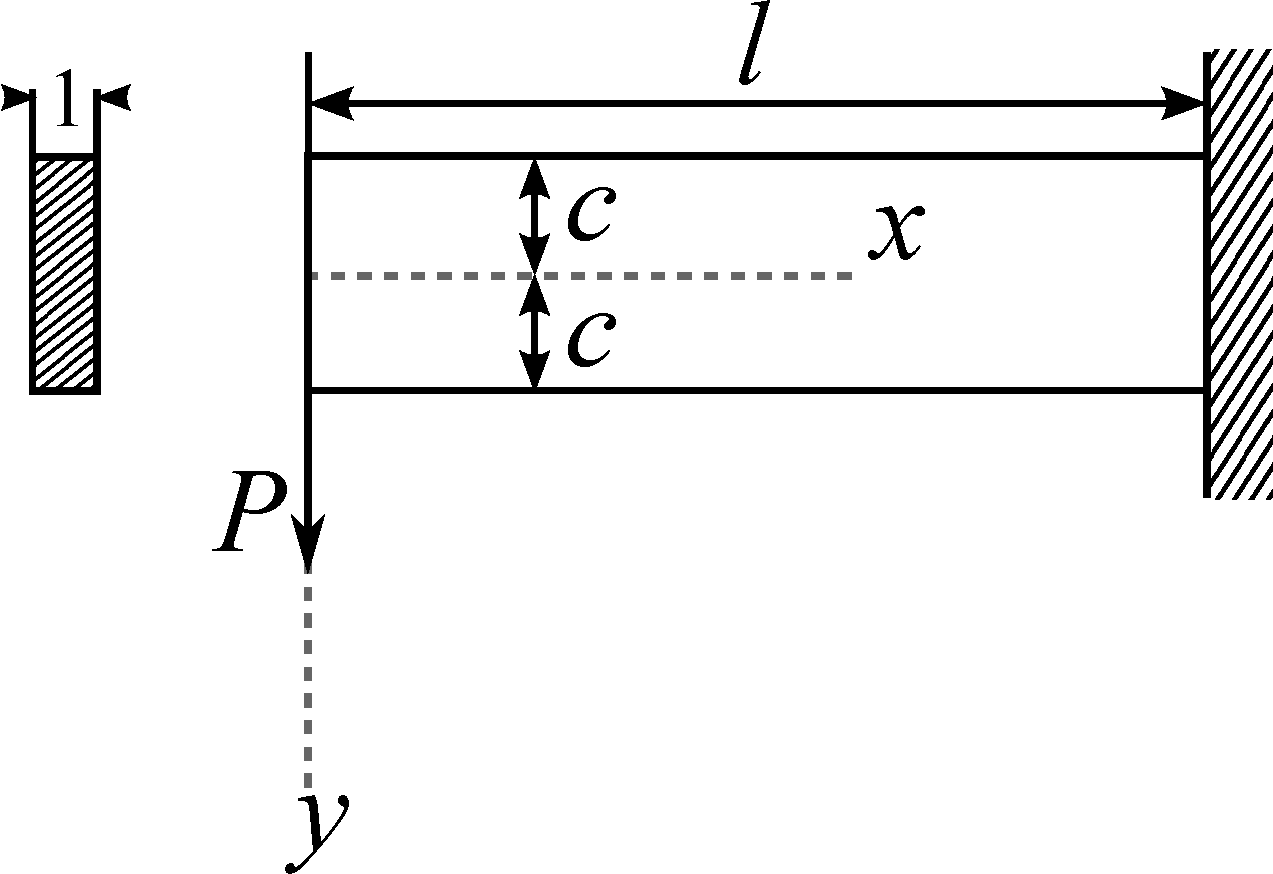
\includegraphics[height=5cm]{Viga_Voladizo.pdf}
	\caption{Viga en voladizo con una carga distribuida en su extremo.}
	\label{fig:viga}
\end{figure}

\begin{enumerate}
\item Determinar las condiciones de frontera del problema.
\item Verificar que las soluciones de esfuerzos y desplazamientos satisfacen las condiciones de frontera.
\item Encontrar la región de la viga que está a compresión y la región tensión, y por tanto el eje neutro. Y determinar la ecuación de desplazamientos para este eje neutro. Comparar con la teoría clásica de vigas.
\end{enumerate}

\item \label{punto05_m} En la  \cref{bloques} se muestra un paralelepípedo de dimensiones $a$, $b$ , $c$, constituido por un material homogéneo elástico y lineal se aloja en una cavidad de la misma forma y dimensiones, cuyas paredes son de un material lo suficientemente rígido para poderlo suponer indeformable.
Sobre la abertura de la cavidad de dimensiones $a\times b$ y a través de una placa rígida de peso y rozamiento despreciables se aplica, perpendicularmente a ella, una fuerza $F$ que comprime al bloque elástico. \footnote{Tomado del ejemplo 3.5 en \cite{book:problemas_resueltos}.}

Calcular:
\begin{enumerate}
\item Las fuerzas laterales ejercidas por las paredes de la cavidad sobre el paralelepípedo;
\item La variación de altura experimentada por el mismo.
\end{enumerate}

\begin{figure}[h]
	\centering
	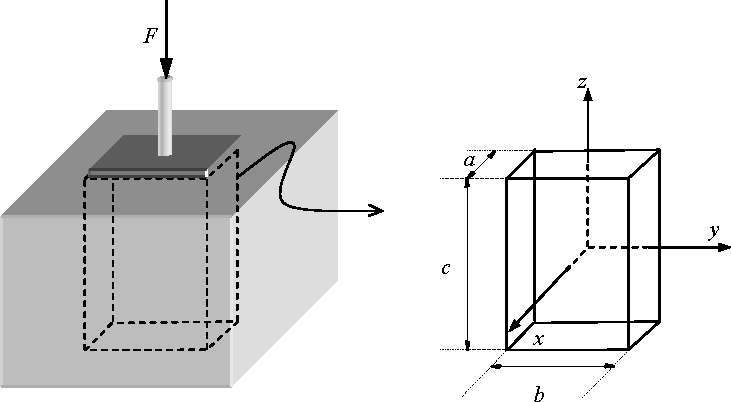
\includegraphics[height=8cm]{bloques.pdf}
	\caption{Paralelepípedo}
	\label{bloques}
\end{figure}

\item \label{punto06_m} En un punto de un suelo que podemos considerar como un sólido elástico lineal se conoce la deformación volumétrica $\epsilon_V = -2\times10^{-3}$ , la deformación tangencial $\epsilon_{xy} = - 3 \times 10^{-3}$ y la deformación  $\epsilon_{xx} = 0$ . El suelo está sometido a un estado de deformación plana en el plano $x y$. Se pide:
\begin{enumerate}
\item Componentes cartesianas del tensor de deformación.
\item  Suponiendo que las constante elásticas son $E = 50$ MPa , $\nu =1/4$ , obtener las componentes del tensor de tensiones y sus valores principales. Obtener asimismo las direcciones en las que las tensiones normales y tangenciales son máximas o mínimas y sus valores.
\end{enumerate}

\item \label{punto07_m} Un sólido se halla sometido a deformación plana, siendo las componentes del tensor de deformación en un punto:
\[\overset{\rightarrow (2)}\epsilon = \left[ \begin{array}{ccc}
-2 & 3 & 0 \\
3 & -10 & 0 \\
0 & 0 & 0
\end{array}  \right] \times 10^{-3}\]
Considere que el sólido tiene un comportamiento elástico lineal e isótropo, definido por
módulo elástico de Young $E = 10$ MPa y coeficiente de Poisson $\nu = 0.25$ .
Se pide:
\begin{enumerate}
\item Obtener las deformaciones principales y las direcciones en que se producen;
\item Obtener las componentes del tensor de tensiones de Cauchy;
\item Obtener las máximas y mínimas tensiones normales;
\item Se sabe que el material rompe cuando en algún plano se alcanza una tensión tangencial
que supere $40$ kPa. Verificar si se produce la rotura.
\end{enumerate}

\item \label{punto08_m}  En la \cref{barcomp}  se muestra una barra, de sección rectangular, $a= 40$ cm, $b = 50$ cm y longitud inicial $L_{c} = 500$ cm, que es  sometida a un ensayo de compresión confinada (está contenida en un recipiente indeformable). En la \cref{bartrac} se muestra una barra, de sección circular, de diámetro $d = 50$ cm y longitud inicial $L_{t} =497$ cm sobre la cual se realiza  un ensayo de tracción simple. Las constantes del material, tanto para la barra rectangular como para la barra circular, son $E=150000$ kgf/cm$^2$ y $\nu=0.20$.

Ambos ensayos se realizan con su extremo fijo  en el plano $z = 0$ y están cargados con un sistema que no transmite esfuerzos cortantes y que hace que el esfuerzo axial se distribuya uniformemente sobre la superficie transversal de las barras. Los esfuerzos que se inducen a las barras varían con el tiempo, conforme a lo mostrado en la  \cref{time}
\begin{figure}[h]
	\centering
	\subfloat[Barra compresión]{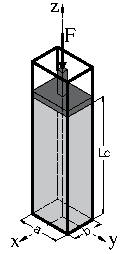
\includegraphics[width=4.0cm]{Compresion.pdf} \label{barcomp}}
	\subfloat[Barra tracción]{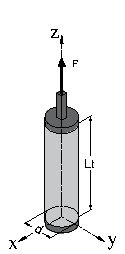
\includegraphics[width=4.0cm]{Traccion.pdf}\label{bartrac}}
	\subfloat[Curvas de esfuerzo]{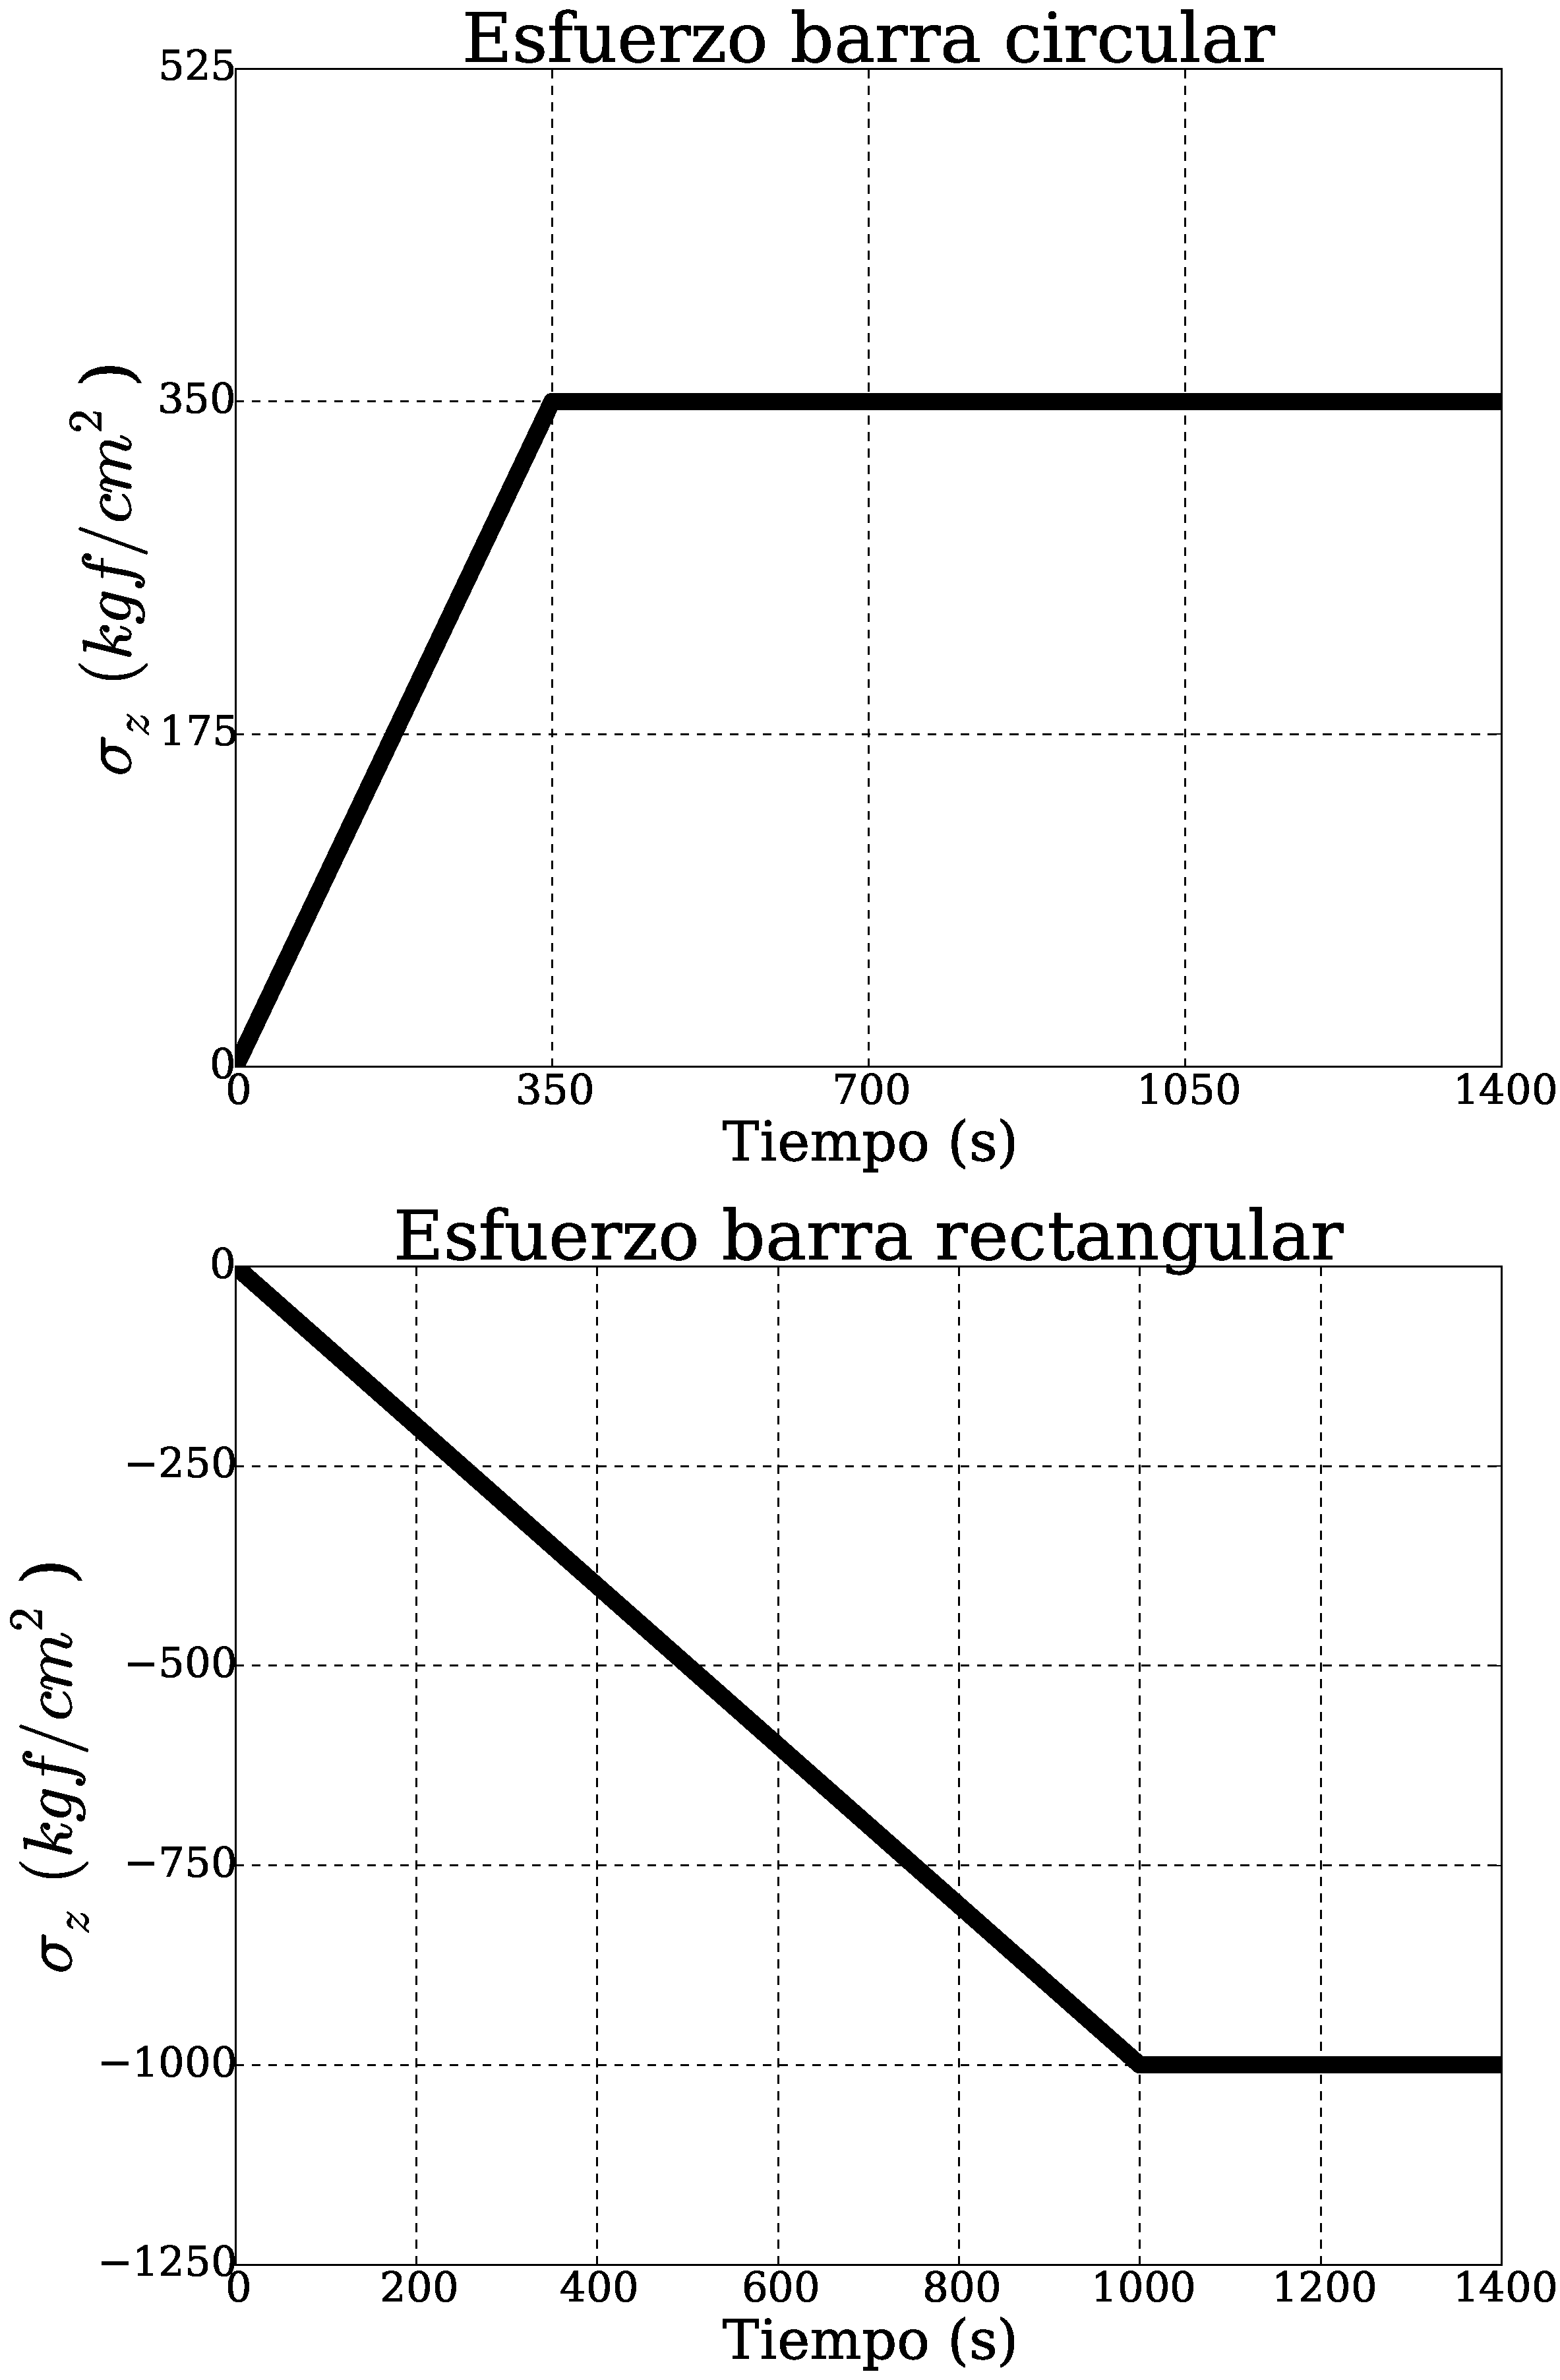
\includegraphics[width=6.0cm]{Esftime.pdf}\label{time}}
	\caption{Esquema ensayos y curvas de aplicación carga}
	\label{ensayo}
\end{figure}

\begin{enumerate}
	\item ¿Cuál es el tiempo $t$ en el cual las dos barras tienen la misma longitud? \\
	\item En la barra circular, ¿cuáles son los desplazamientos $u$, $v$ y $w$ y las deformaciones $\varepsilon_{xx}$ $\varepsilon_{yy}$ y $\varepsilon_{zz}$ en el punto de coordenadas $(x,y,z) = (20,15,450)$ cm para el tiempo $t = 300$ s?
	\item ¿Cuál es el valor del máximo esfuerzo cortante en un punto al interior de la barra rectangular durante el ensayo?
	\item  ¿Cuál es el área mínima que alcanza la sección transversal de la barra circular durante el ensayo?
	\item  ¿En la barra rectangular, en el tiempo $t=1000$ s cuál son las fuerzas $F_x$ y $F_y$ que le transmite la barra a las paredes del recipiente?
\end{enumerate}

\item En la \cref{placa} se presenta una placa en forma de rombo sometida a la acción de una carga, en el plano $XY$, que se encuentra distribuida sobre su perímetro y cuyo campo de desplazamientos está dado por:
\[u \left(x,y,z \right) =  \dfrac{A}{E}  \left(1 - \nu \right) x,\quad
v \left(x,y,z \right) = \dfrac{A}{E}  \left(1 - \nu \right) y,\quad
w \left(z \right) = -\dfrac{2A \nu}{E} z\]
con $A$ una constante positiva, $E$  el módulo de elasticidad del material y $\nu$ la relación de Poisson.
\begin{figure}[h]
	\centering
	\subfloat[Placa]{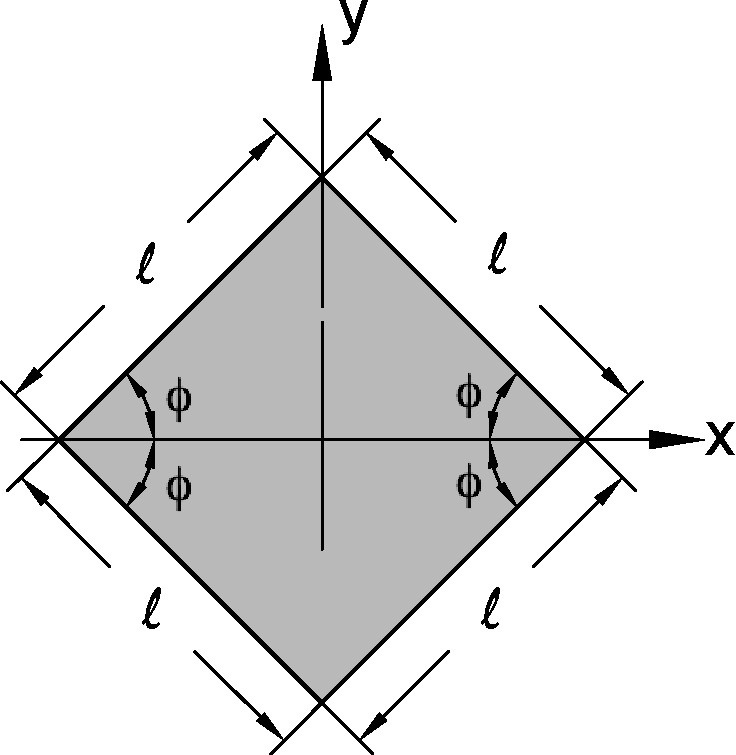
\includegraphics[width=2.5in]{cuna.pdf}\label{placa}}
	\hspace{2 cm}
	\subfloat[Esquema para dibujar las cargas axiales y tangenciales]{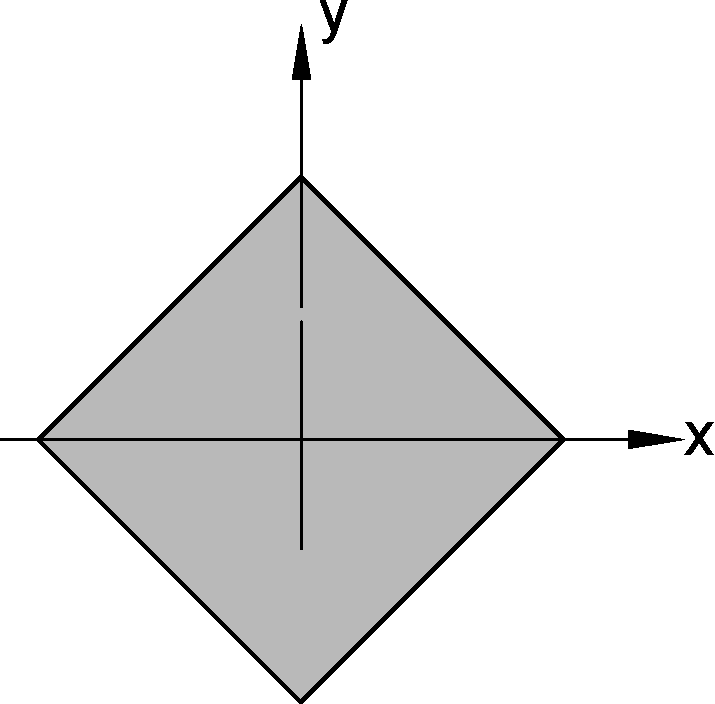
\includegraphics[width=2.5in]{cunanada.pdf}\label{esquema}}
	%\label{placa}
\end{figure}

\begin{itemize}
	\item Determine la deformación unitaria axial máxima $\varepsilon$ y la deformación angular máxima $\gamma$ que se presentan en la placa ¿En qué puntos se presentan?.
	\item Dibujar la configuración deformada de la placa en el plano $xy$ ¿Cuáles son los puntos que experimentan los mínimos desplazamientos?.
	\item Ilustre la deformación de la partícula con coordenadas $\left( \dfrac{l}{4}, 0, 0 \right)$ en el plano $xy$. Utilice cuadrados de tamaño diferencial.
	\item Determine y represente gráficamente, sobre la figura (b), la tensión normal y tangencial a la cara de la placa, contenida en el cuadrante I del plano $XY$.
\end{itemize}

\end{enumerate}

\end{document}
